\documentclass[10pt,a4paper]{article}

\usepackage{polski}
\usepackage[polish]{babel}
\let\lll\undefined
\usepackage[utf8]{inputenc} 
\usepackage{amsmath}
\usepackage{amssymb}
\usepackage{graphicx}
\usepackage{wrapfig}
\usepackage{amsthm}
\newtheorem{theorem}{Twierdzenie}
\title{Clustering}
\author{Tomasz Kulik}
\date{}
\begin{document}
\maketitle

\begin{abstract}
W dokumencie przedstawiona została podstawowa analiza złożoności obliczeniowej problemu analizy skupień z ograniczeniami -
znajdowania podziału zbioru na trzy podzbiory, w których odległość między każdą parą elementów danego zbioru
jest ograniczona przez stałą. Omówione zostały również inne warianty ograniczeń i ich wpływ na przynależność
problemów do poszczególnych klas złożoności obliczeniowych.
\end{abstract}

\section{Wstęp}\label{sec:wstep}
\par
Grupowanie jest problemem optymalizacyjnym polegającym na podzieleniu zbioru danych wejściowych na zadaną liczbę
rozłącznych podzbiorów minimalizując przy tym funkcję celu. Analiza skupień z ograniczeniami (z ang. Constrained
Clustering) jest wariantem powyższego problemu, w którym wprowadza się dodatkowe ograniczenia na zadane pary
elementów ze zbioru wejściowego. Przeanalizowany został problem podziału zbioru danych wejściowych na 3 rozłączne
podzbiory tak, aby dla każdych dwóch elementów należących do danego podzbioru odległość między nimi była ograniczona
z góry przez stałą. Praca ta skupiona jest zarówno na problemie znajdowania zbioru rozwiązań dopuszczalnych,
tj. spełniających ograniczenia jak i na kwestii optymalizacyjnej.

\section{Opis problemu}\label{sec:problem}
Dla danych wejściowych:
\begin{equation}
	\begin{aligned}
    X & - \text{zbiór skończony} \\
    B & - \text{stała} \\
    d(x,y) &- \text{metryka na zbiorze X}
    \end{aligned}
\end{equation}
należy wyznaczyć trzy rozłączne podzbiory zbioru X
\begin{equation}
	\{ X_{1}, X_{2}, X_{3} \}
\end{equation}
gdzie
\begin{equation}
	\forall_{x,y \in X_{i}} \; d(x, y) \leq B
\end{equation}

\begin{theorem}
Problem podziału zbioru na trzy rozłączne podzbiory zachowując powyższe ograniczenia jest NP-zupełny.
\end{theorem}
\begin{proof}
Niech $G = (V, E)$ będzie grafem z problemu 3-kolorowania, gdzie $V$ jest zbiorem wierzchołków, a $E$ to zbiór krawędzi.
Dodatkowo niech $G' = (V, E')$ będzie dopełnieniem grafu $G$, a każda z krawędzi $(x, y) \in E'$ niech oznacza
spełnienie relacji $d(x, y) \leq B$ z problemu podziału na 3 rozłączne podzbiory z ograniczeniem odległości.
Można zauważyć, że znalezienie takiego trójkolorowania grafu $G$ - $(X_1, X_2, X_3)$ skutkuje znalezieniem
trzech rozłącznych pozbiorów wierzchołków w grafie $G'$. Każdy ze wspomnianych podzbiorów musi być kliką w grafie $G'$,
ponieważ w grafie $G$ żaden z wierzchołków o tym samym kolorze nie mógł być połączony krawędzią. Z założenia w grafie $G'$
istnienie krawędzi pomiędzy dwoma wierzchołkami oznacza spełnienie warunku odległości, co oznacza że odległość
pomiędzy każdymi dwoma wierzchołkami w takich podzbiorach jest mniejsza od $B$. W rezultacie daje to trzy
rozłączne podzbiory, które należało znaleźć.
\par
Z drugiej strony stwierdzenie, że graf $G$ nie jest 3-kolorowalny implikuje brak możliwości podziału wierzchołków
grafu $G'$ na trzy podzbiory zachowując (3). To oznacza, że problem 3-kolorowania redukuje się
w czasie wielomianowym do problemu, na którym skupia się ten referat. Powyższa redukcja dowodzi NP-zupełności.
\end{proof}

\section{Przykłady}
\par
Poniżej znajdują się dwa przykłady działania algorytmu podziału wierzchołków grafu na 3 podzbiory. Krawędzie grafu
oznaczają, że warunek odległości pomiędzy daną parą wierzchołków został spełniony i mogą (ale nie muszą)
znajdować się w jednym klastrze. Jeśli krawędź nie wystąpiła pomiędzy wierzchołkami to znaczy, że ich odległość
wykluczała znalezienie się w jednym klastrze. Innymi słowy w danym podzbiorze wynikowym pomiędzy wszystkimi jego
wierzchołkami musi istnieć krawędź. Każdy taki podzbiór jest kliką.

\subsection{Negatywny przypadek}\label{sec:negatywny}
\par
W tym przypadku nie jest możliwe znalezienie takich 3 rozłączych podzbiorów wierzchołków grafu.
Najmniejsza liczba podzbiorów dla poniższego grafu wynosi 4.

\begin{center}
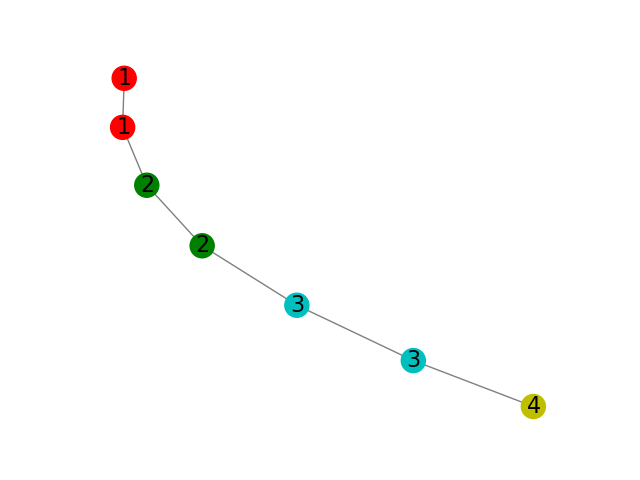
\includegraphics[width=0.75\textwidth]{negatywny.png}
\end{center}

\newpage
\subsection{Pozytywny przypadek}\label{sec:pozytywny}
W grafice przedstawiono graf, którego węzły skutecznie podzielono na 3 rozłączne podzbiory. Łatwo zauważyć, że
rozwiązanie tego problemu prowadzi do podzielenia grafu na trzy kliki.

\begin{center}
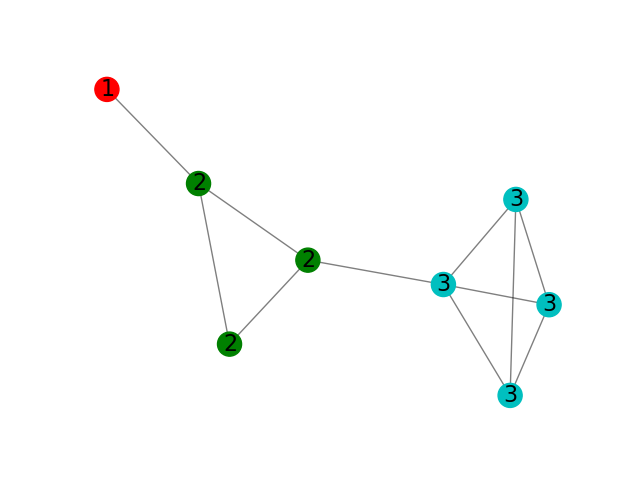
\includegraphics[width=0.75\textwidth]{pozytywny.png}
\end{center}

\section{Warianty}\label{sec:warianty}
\par
Istnieją również inne warianty ograniczeń jakie można nałożyć na elementy dzielonego zbioru.
Są to między innymi:
\begin{itemize}
  \item $CannotLink(x, y)$ - węzły x oraz y nie mogą przynależeć do tego samego klastra. Warto zauważyć, że
        problem trójpodziału zbioru ze względu na odległości można zamodelować przy pomocy tego ograniczenia.
        Wystarczy dla każdej pary $(a, b)$ leżącej dalej niż $B$ nałożyć $CannotLink(a, b)$. Stąd w ogólności
        problemy k-podziału z ograniczeniami $CannotLink$ są NP-zupełne.
	\item $MustLink(x, y)$ - węzły $x$ oraz $y$ ze zbioru $X$ muszą znaleźć się w jednym klastrze.
  \item $\delta-Constraint$ - dla każdej pary $(x,y)$ elementów zbioru $X$ jeśli $d(x,y) < \delta$ to $x$ i $y$ muszą
        znaleźć się w jednym klastrze. Innymi słowy dla odpowiednio bliskich elementów należy nałożyć ograniczenie
        $MustLink$, a parametr $\delta$ wyznacza tą odległość.
  \item $\epsilon-Constraint$ - jeżeli w klastrze znajduje się więcej niż jeden węzeł to dla każdego węzła $s$ w klastrze
        musi znajdować się przynajmniej jeden węzeł $t$, który spełnia warunki $\epsilon-neighbor$, tj.
        jeśli $d(s,t) \leq \epsilon$. Parafrazując, dany element $s$ może przynależeć do podzbioru $X_i$ tylko wtedy,
        gdy choć jeden inny element należący do $X_i$ znajduje się w odległości co najwyżej $\delta$ od elementu $s$.
        Wyjątek stanowi jednoelementowy podzbiór, dla którego nie rozpatruje się tego warunku.
\end{itemize}

\begin{table}
\caption{Warianty problemu analizy skupień dla dancyh kombinacji ograniczeń}
\begin{tabular}{|| c | c | c ||}
    \hline\hline
  Kombinacja ograniczeń & Zadana liczba podzbiorów & Dowolna liczba podzbiorów \\
    \hline\hline
  $CannotLink$ & NP-zupełny & P \\
    \hline
  $MustLink$ i $\delta -Constraint$ & P & P \\
    \hline 
  $CannotLink$ i $\epsilon -Constraint$ & NP-zupełny & P \\
    \hline 
  $\delta -Constraint$ i $\epsilon -Constraint$ & P & P \\
    \hline 
  Wszystkie powyższe & NP-zupełny & NP-zupełny \\
    \hline\hline
\end{tabular} 
\end{table}


\section{Wariant optymalizacyjny}\label{sec:opt}
\par
Powyżej przedstawiono wariant decyzyjny problemu analizy skupień. W celu zbadania wariantu optymalizacyjnego należy
rozpatrzeć minimalizację parametru $B$, tj. wskazania takiej najmniejszej odległości pomiędzy elementami danego klastra,
dla której zachodzi warunek podzielności na 3 rozłączne podzbiory.

\begin{equation}
  min \; B
\end{equation}

tak, aby spełnić ograniczenia:

\begin{equation}
  \left\{
    \begin{aligned}
      &X_1 \cup X_2 \cup X_3 = X \\
      &X_1 \cap X_2 = X_1 \cap X_3 = X_2 \cap X_3 = \emptyset \\
      &\forall_{X' \in \{ X_1, X_2, X_3 \}} \; \forall_{x,y \in X'} \; d(x, y) \leq B
    \end{aligned}
    \right.
\end{equation}


\section{Bibliografia}\label{sec:bibliografia}
[1] C. M. Emre. Feasibility Issues [W:] \textit{Unsupervised Learning Algorithms}, 
    Springer International Publishing AG, 2016. \par\noindent
[2] I. Davidson, S. S. Ravi. \textit{Clustering With Constraints: Feasibility Issues and the k-Means Algorithm},
    DOI: 10.1137/1.9781611972757.13, Źródło: DBLP, 2005.

\end{document}